% 2022 新高考Ⅱ卷 11：正方形 ABCD 与同侧两条垂线 DE、BF
% 取 AB=2，立体坐标 A(0,0,0)、B(2,0,0)、C(2,2,0)、D(0,2,0)，DE⊥平面 ABCD 且 DE=2，
% BF⊥平面 ABCD 且 BF=1，即 E(0,2,2)、F(2,0,1)。
% 画布投影：(x,y,z) -> x·(1,0) + y·(0.42,0.30) + z·(0,1)。
% 虚线（被遮挡）：CD、DA、AC、DE；其余为可见实线。
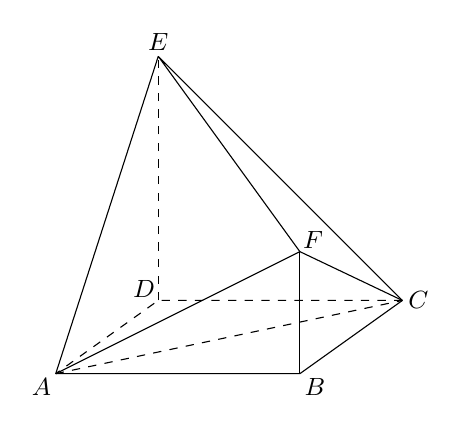
\begin{tikzpicture}[scale=1.55, font=\small]
  \coordinate (A) at (0,0);
  \coordinate (B) at (2,0);
  \coordinate (C) at (2.84,0.60);
  \coordinate (D) at (0.84,0.60);
  \coordinate (E) at (0.84,2.60);
  \coordinate (F) at (2,1.00);
  % 可见实线
  \draw (A) -- (B) -- (C);
  \draw (B) -- (F);
  \draw (E) -- (A)  (E) -- (C)  (E) -- (F);
  \draw (F) -- (A)  (F) -- (C);
  % 被遮挡
  \draw[dashed] (C) -- (D) -- (A);
  \draw[dashed] (A) -- (C);
  \draw[dashed] (D) -- (E);
  \node[below left,  inner sep=1.5pt] at (A) {$A$};
  \node[below right, inner sep=1.5pt] at (B) {$B$};
  \node[right,       inner sep=2pt]   at (C) {$C$};
  \node[above left,  inner sep=1pt]   at (D) {$D$};
  \node[above,       inner sep=2pt]   at (E) {$E$};
  \node[above right, inner sep=1pt]   at (F) {$F$};
\end{tikzpicture}
